\documentclass[11pt]{article}
\usepackage[left=2cm,right=1.5cm,bottom=2cm,top =2cm]{geometry}                % See geometry.pdf to learn the layout options. There are lots.
\usepackage{amsmath}
\geometry{letterpaper}   
                % ... or a4paper or a5paper or ... 
%\geometry{landscape}                % Activate for for rotated page geometry
%\usepackage[parfill]{parskip}    % Activate to begin paragraphs with an empty line rather than an indent

\usepackage{graphicx}
\usepackage{amssymb}
\usepackage{epstopdf}
\DeclareGraphicsRule{.tif}{png}{.png}{`convert #1 `dirname #1`/`basename #1 .tif`.png}

\usepackage[most]{tcolorbox}
\usepackage{xcolor}
\definecolor{vlightgray}{rgb}{0.9,0.9,0.9}

\title{Workshop \#: IVPs with PDEs and Spectral Methods \\ The  Schrodinger Equation }
\author{\textbf{Reading:} Numerical Recipes, Ch. 20.7 (\& Sec. 20.2.1)}
\date{}                                           % Activate to display a given date or no date

\begin{document}
\maketitle

In quantum physics, a particle is described by a (complex) wavefunction $\psi(x,t)$. The evolution of the wavefunction is given by the Schrodinger equation
\begin{align}
i \hbar \frac{\partial \psi (x,t)}{\partial t}  &= \hat H  \psi(x,t) & \hat H &= \hat T + \hat V  =   -\frac{\hbar^2 }{2m} \frac{
\partial^2}{\partial x^2} + V(x)
\end{align}
where $\hbar$ is Planck's constant and $m$ is the particle mass. The Hamiltonian operator $\hat H$  consists of the kinetic energy operator $\hat T$ and the external potential $V(x)$. Aside from quantum physics, Schrodinger-type equations (including nonlinear versions) also arise in areas such as optics and hydrodynamics. This worksheet covers some key techniques for solving them numerically using spectral methods.

\section{Particle in a Ring (walkthrough / demonstration)}
First consider the dynamics of a particle in a ring-shaped trap of radius $R$. This can be modelled using the 1D Schrodinger equation with $V(x) = 0$ and periodic boundary conditions.
\begin{enumerate}
%\item Taylor expand the potential about the minimum, and show it can be approximated as a harmonic oscillator potential of the form $V(x) \approx \tfrac{1}{2} m \omega^2 x^2 $ where $\omega = \sqrt{2 V_0 / m \sigma^2}$

   

\item \textbf{Nondimensionalization}: By defining appropriate dimensionless variables (denoted by tildes) 
%\begin{align}
%\tilde x &= x / \ell, & \tilde t  &= t / \tau & \tilde \psi &= \psi /\sqrt{\ell},
%\end{align} 
we can show that the  Schrodinger equation becomes
\begin{align}
i \frac{\partial \tilde \psi}{\partial  \tilde t} = - \frac{1}{2} \frac{\partial^2 \tilde \psi} {\partial \tilde x^2}.
\end{align} 

%\item \textbf{Dynamics:} If we apply the Fourier transform to the Schrodinger equation, we have
%\begin{align}
% \frac{\partial \psi(k,t)}{\partial t} = -\frac{ik ^2 }{2} \psi(k,t) 
%\end{align}
%giving the wavefunction at time $t$ in Fourier space as
%\begin{equation}
% \psi(k,t) = \exp[-i k^2 t /2 ] \psi(k,0).
%\end{equation}
\item \textbf{Dynamics:} The Fourier transform gives us a simple procedure for finding the wavefunction at any time $t$ by simply hopping between position space and wavenumber space:
%\begin{equation}
%\psi(x, t) = \mathcal{F}^{-1} \{ e^{-i k^2  t /2}   \mathcal{F}[\,\psi(x,0) \, ] \, \}
%\end{equation}
%Or, diagramatically:
\begin{figure}[!h]
\centering
\hspace{1cm}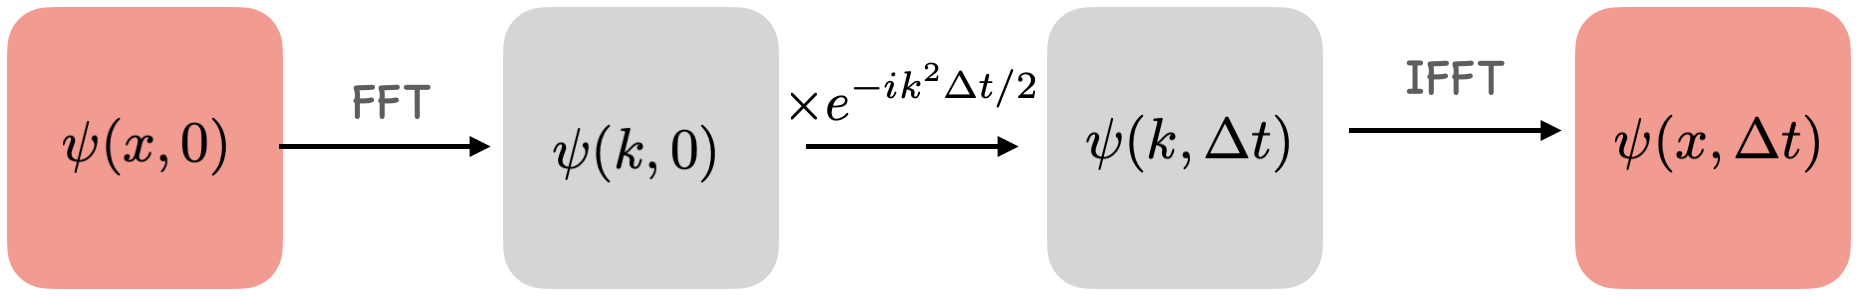
\includegraphics[width= 0.6\columnwidth]{algorithm2.png}
\end{figure}

\item   \textbf{Compile and Run:} Code to solve the free space dynamics is provided in the file  \fcolorbox{white}{vlightgray}{\texttt{\color{magenta}{schrodinger.cpp}}}. Familiarize yourself with the code, and the corresponding \fcolorbox{white}{vlightgray}{\texttt{\color{magenta}{makefile}}}.  To complile the program,  simply type \fcolorbox{white}{vlightgray}{\texttt{\color{magenta}{make}}} into the command line. 

\item \textbf{Analyse:} Simulate the dynamics of a gaussian wavepacket $\psi(x,0) = 1/(\pi \sigma^2)^{1/4} \exp(-x^2/2\sigma^2)$ with $\sigma \ll  R $. Make a plot of the probability amplitude $|\psi(x,t)|^2$ for several time instances $t$. Modify the code to calculate and save the variance of the particles position 
\begin{equation}
\langle x^2(t) \rangle = \int dx\;   x^2  |\psi(x,t)|^2
\end{equation} 
Plot $\langle x^2 \rangle$ vs $t$  and comment on the result. 
\end{enumerate}
\section{Harmonic Oscillator Potential (student exercise)}
 Now consider the harmonic oscillator,
\begin{equation}
V(x) = \tfrac{1}{2} m \omega^2 x^2.
\end{equation}
\begin{enumerate}
\item \textbf{Dimensionless variables:}  As above, we can work with dimensionless variables by writing  $\tilde x = x / \ell$, $\tilde t  = t / \tau$, $\tilde \psi = \psi /\sqrt{\ell}$.  Show that the Schrodinger equation can be written (dropping the tildes) in the dimensionless form 
\begin{equation}
i \frac{\partial \psi(x,t)}{\partial t} = \left[ -\frac{1}{2} \frac{\partial^2 }{\partial x^2} + \frac{1}{2} x^2 \right ] \psi(x,t)
\end{equation}
Find expressions for $\tau$ and $\ell$. What (physically) do these parameters correspond to? 



\item \textbf{Algorithm:} To extend our program to deal with the potential, we will make use of the \emph{Split Operator Method}. As before, the wavefunction at any time $t +\Delta t$ is  given exactly by
\begin{equation}
\psi(x, t+\Delta t) = \exp\left[- i ( \hat T + \hat V)\Delta t  \right] \psi(x,t). 
\end{equation}
To perform the evolution purely  in either $x$- or $k$-space, we would have to evaluate one of the operators as a (costly) matrix exponential. However, for a small step $\delta t$, then we may write 
\begin{equation}
\exp\left[- i (\hat T + \hat V) \delta t  \right] \approx \exp \left[ - i \hat T \delta t  \right] \exp \left[ - i \hat V \delta t  \right]  + \mathcal{O}(\delta t)^2.
\end{equation}
Modify the program to implement the split operator method. 

\item \textbf {Dynamics:} Suppose a particle is initially in the ground state of the well, with $\psi(x) = (1/\pi)^{1/4}\exp{[-x^2/2]}$, and the trap is then suddenly displaced by a distance $a=1$. Simulate the dynamics and calculate
\begin{align}
\langle x(t) \rangle &= \int dx\; x |\psi(x)|^2  & \langle p(t) \rangle = \int  \ dk\; k |\psi(k)|^2
\end{align}
Do the same for a case where instead the trap frequency is suddenly changed to $\omega' = 0.5 \omega$ and calculate $\langle x^2(t) \rangle$ and $\langle p^2(t) \rangle $.
 \item \textbf {Groundstate using imaginary time:} The same techniques for dynamics can be used to find the groundstate of any potential. The trick is to make the replacement 
$ t \rightarrow -i t$. Since eigenstates satisfying $ \hat H \phi_n = E_n \phi_n$ normally evolve as
 \begin{equation}
 \phi_n(x,t) = e^{-i E_n t }\phi_n(x),
  \end{equation} 
each state will decay at a rate proportional to its energy under imaginary time evolution.  Any wavefunction can be decomposed into the eigenstates, since they form a complete basis:
\begin{equation}
\psi(x,t) = \sum_n c_n(0) e^{-i E_n t} \phi_n(x).
\end{equation}
It follows that any intial guess (as long as it doesn't have  \emph{zero} overlap with $\phi_0$) will eventually be dominated by groundstate, since it decays at the slowest rate. If we renormalize the wavefunction after each timestep: 
\begin{equation}
\psi(x) \rightarrow \frac{\psi(x)}{  \left( \textstyle{\int{|\psi(x')|^2} dx'} \right) },
\end{equation}
 we maintain the condition $\int |\psi(x)|^2 dx =1$, and will obtain the correctly normalized groundstate. Modify your code to solve for the groundstate of the potential.

%\begin{equation}
%\delta V(x) = V_0 \exp(-x^2/\sigma^2)
%\end{equation}
%is added near the trap centre. Simulate the dynamics and calculate the probability of finding the particle to the right of the barrier 
%\begin{equation}
%P_R(t) = \int_0^{L/2} dx\; |\psi(x,t)|^2  
%\end{equation}
%for several values of $V_0$ and plot them vs $t$. Make a plot or table of $\max[P_R]$ vs $V_0$ for $V_0 = \{0, 10, 20, .. 100\}$.

\end{enumerate}

%\newpage
%\section{A Nonlinear BVP with Shooting }
%The Poisson-Boltzmann equation is an equation that appears in a variety of systems such as electron plasmas, polymers, and hydrodynamics. It relates the density of charges $n(\mathbf{r})$ and the to a  potential field $\phi(\mathbf{r})$
%\begin{equation}
%n(\mathbf{r})  =  n_0\exp\{-\beta\phi(\mathbf{r}) -  \alpha r^2 \}
%\end{equation}
%\begin{equation}
%n(\mathbf{r}) = -\nabla^2{\phi(\mathbf{r})}
%\end{equation}
%Since the PB equation is a  \emph{nonlinear} partial differential equation, in general it must be solved numerically,  analytically and it must be solved numerically.  
%
%\begin{enumerate}
%\item Defining $u(r) = \log{[n(r)/n_0]}$, show the equation can be written as 
%\begin{align}
% u''(r) + \frac{1}{r} u'(r)  &= f e^{u} - g, & u(0) &=0, \quad u'(0) = 0.
%%\nabla^2 \log{\left[ \frac{n (r)}{n_0}\right]}  =  \nabla^2 (-\beta \phi(r) - \beta \omega r^2 )
%\end{align}
%Give expressions for $f$ and $g$.
%\end{enumerate}

%\section{}
%\subsection{}



\end{document}  